\documentclass[12pt, a4paper, oneside]{report}

\usepackage{amsmath}
\usepackage{esint}
\usepackage{geometry}
\usepackage{graphicx}
\usepackage{subcaption}
\usepackage{cleveref}
\usepackage{ctex}
\usepackage{listings}
\usepackage{color}
\definecolor{dkgreen}{rgb}{0,0.6,0}
\definecolor{gray}{rgb}{0.5,0.5,0.5}
\definecolor{mauve}{rgb}{0.58,0,0.82}
\lstset{frame=tb,
	language=Python,
	aboveskip=3mm,
	belowskip=3mm,
	showstringspaces=false,
	columns=flexible,
	basicstyle={\small\ttfamily},
	numbers=left,%设置行号位置none不显示行号
	numberstyle=\tiny\color{gray},
	keywordstyle=\color{blue},
	commentstyle=\color{dkgreen},
	stringstyle=\color{mauve},
	breaklines=true,
	breakatwhitespace=true,
	escapeinside=``,%逃逸字符(1左面的键),用于显示中文例如在代码中`中文...`
	tabsize=4,
	extendedchars=false %解决代码跨页时,章节标题,页眉等汉字不显示的问题
}
% 导言区

\title{Report 1: Poisson Image Editing}
\author{Chihao Shen 121020163}
\CTEXoptions[today=old]
\geometry{left=2cm,right=2cm,top=2.5cm,bottom=2.5cm}



\begin{document}
	
	\rmfamily
	\maketitle
	
	\songti 
	
	\section{任务描述}
	采用泊松图片编辑原理融合图片,结果是形成一张前景与背景色调相似,融合恰当的图片。采用梯度混合原理,保留背景图片的大致细节,又不失前景的细节。
	
	\centerline{	
		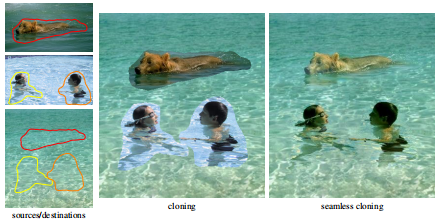
\includegraphics[scale=0.6]{task.png}
	}
	\section{理论基础}
	\subsection{基本Poisson Image Editing}
	要将源图像融合至目标图像上,我们先作如下定义:
	
	\noindent $g$:源图像选中部分,已知。
	
	\noindent $\textbf{v}/\nabla g$:源图像的梯度向量场,已知。
	
	\noindent $\nabla f$:融合图像的梯度向量场,未知。
	
	\noindent $S$:目标图像,其二维标量场构成的函数为$f^*$,已知。
	
	\noindent $\Omega$:目标区域,其二维封闭标量场构成的函数为$f$,未知,是要求解的量。
	
	\noindent $\partial\Omega$:融合区域边界,选已知量$f$在边界上的值,已知。
	
	\centerline{	
		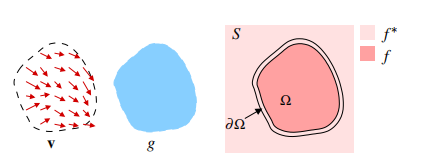
\includegraphics[scale=0.8]{task2.png}
	}
	
	图片的纹理是由梯度$\nabla$决定的,而色调则是由像素值决定的。要尽可能地保留源图像的纹理,我们需要最小化融合后区域和源图像区域各个像素梯度差值的和,即$$\min\limits_{f}^{}\iint\limits_{\Omega}\left|\nabla f - \nabla g\right|^2$$
	
	要让色调相同,则边界的值应和目标图像对应像素的值相同,即$$f|_{\partial\Omega} = f^*|_{\partial\Omega}$$
	
	根据拉格朗日方程,要使梯度差值尽可能小,则源图像与目标图像对应位置的散度$\Delta$应该相同(具体证明过程详见参考内容,这里不给出具体证明过程),即$$\Delta f = \Delta g$$
	
	由于图像是由离散的像素点构成的,其散度可用拉普拉斯算子表示,其卷积核为$$\left[\begin{array}{ccc}
		0 & 1 & 0\\
		1 & -4 & 1\\
		0 & 1 & 0
	\end{array} 
	\right]$$
	
	若简化模型,假设有一张$4\times4$的图像$\left[\begin{array}{cccc}
		x1 & x2 & x3 & x4\\
		x5 & x6 & x7 & x8\\
		x9 & x10 & x11 & x12\\
		x13 & x14 & x15 & x16
	\end{array}\right]$,$xi$表示各个位置的像素值,则由于各个像素点散度相等,我们用拉普拉斯卷积核扫描中间四个像素,能给出四个线性方程。尽管看似有12个未知量,但由于边界是已知的,实际未知量只有$x6, x7, x10, x11$四个,因此将已知常数化至右侧,四个不等价的线性方程与四个未知数,最终能够化成$$Ax=b$$的形式。通过高斯消元解得每一个未知数,推广至一般图像,我们能够获取每个待定像素的像素值。将其填充至目标图像,就能够获取融合后的图像。
	\subsection{Mixing Gradient}
	在泊松融合基础上,有些图像要求保留背景图像的纹理细节,那么通过比较源图像和目标图像对应像素的梯度值,保留较大值,取代源图像的梯度值,即
	$$\nabla g = \begin{cases}
	\nabla f^*  \qquad if |\nabla f^*| > |\nabla g|, \\
	\nabla g \qquad else.	\end{cases}$$

	在实际操作过程中,我们可以在计算拉普拉斯算子四个方向时先比较和改变对应梯度大小,再计算拉普拉斯算子值,无需先对源图像进行操作。
	\section{代码实现}
	\subsection{代码说明}
	\noindent 库:numpy, OpenCV, sparse
	
	其中OpenCV用于获取和展示图片,尽管OpenCV有自带的API可以直接实现泊松图片编辑的效果,但这里还是给出其源代码,还原算法过程。
	
	numpy用于存放较简单的数列。图像也是用ndarray的形式存放的。
	
	sparse用于创建稀疏矩阵和实现高斯消元。在实现线性方程组高斯消元时,我们发现像素较大的图片若用ndarray存放拉普拉斯算子,一方面会大量增加冗余的空间复杂度,另一方面当像素达到一定程度时,numpy会提示溢出边界的报错,因此采用numpy计算不是十分方便。此外,用numpy存放拉普拉斯算子需要遍历矩阵,同样也会增加时间复杂度,而sparse则只须定位坐标并填入值。笔者的同学采用numpy渲染一张图需要7秒,而采用sparse则只需要4秒,大大降低了时间复杂度。
	
	本代码需要给出一张源图像,一张与源图像相同的掩膜,一张大于源图像的目标图像以及融合在目标图像上的源图像左上角的坐标位置。若该坐标使得源图像超出目标图像轮廓范围,则给出超出范围的提示。
	
	本代码有一个漏洞,即掩膜的锚点区域不能涵盖掩膜的边界。为了节省内存空间,拉普拉斯算子提取的是源图像各个方向的像素值,代码中没有给出扩展后的图像,因此对于边界的锚点,方向会按3进行计算,少加了一份锚点的值,使得结果图偏暗。我们将源图像改为扩展后的图像就不会出现此类问题,这里不给出改进方案。
	
	在实际操作中发现,对于一些特定的图像,泊松图片编辑也不能够给出很好的融合,仍然会出现部分区域偏亮或偏暗的情况。(原以为是代码的问题,操作后发现无论是下列代码还是OpenCV给出的API都会出现这种情况。)
	
	\subsection{基本Poisson Image Editing代码}
	
	\begin{lstlisting}
import scipy.sparse.linalg as splinalg
import scipy.sparse as sparse
import numpy as np
import cv2
import time

# 泊松图像编辑函数
"""
(p_start_x, p_start_y):源图像左上角像素的坐标
p_mask:掩膜图像,必须是双通道的,大小和源图像相同
p_tgt:目标图像
p_src:源图像,必须比目标图像小或相等
"""


def poisson_image_editing(p_start_y, p_start_x, p_mask, p_tgt, p_src):
	mask_row, mask_col = p_mask.shape[0], p_mask.shape[1]  # 掩膜的宽度和长度
	tgt_row, tgt_col = p_tgt.shape[0], p_tgt.shape[1]  # 目标图像的宽度和长度
	
	# 判断:源图像映射在目标图像上是否超出了目标图像边界
	if p_start_y + mask_row > tgt_row or p_start_x + mask_col > tgt_col:
		# 提示并返回目标图像
		print('Out of range!')
		return p_tgt
	else:
		p_src = np.array(p_src, np.float32)  # 位深改为浮点数,防止np.uint8超出255后归零,下同
		
		# 按源图像左上角像素的坐标重建和目标图像大小相同的掩膜和源图像
		# 注意掩膜的通道数为2
		new_mask = np.zeros([tgt_row, tgt_col], np.float32)
		new_src = np.zeros([tgt_row, tgt_col, 3], np.float32)
		new_mask[p_start_y:p_start_y + mask_row, p_start_x:p_start_x + mask_col] = p_mask
		new_src[p_start_y:p_start_y + mask_row, p_start_x:p_start_x + mask_col] = p_src
		
		# 获取新掩膜和原掩膜每个锚点的坐标
		# 纵坐标存于pix_y,横坐标存于pix_x,一一对应
		pix_y, pix_x = np.where(new_mask)
		pix_old_y, pix_old_x = np.where(p_mask)
		
		pix_sequence = np.zeros([tgt_row, tgt_col])  # 创建和目标图像大小相同的全黑模板
		pix_sequence[pix_y, pix_x] = np.arange(pix_y.shape[0])  # 模板上每个掩膜的锚点按从上到下,从左到右的顺序依次标上序号
		
		direction = [[-1, 0], [1, 0], [0, -1], [0, 1]]  # 拉普拉斯算子的四个方向
		
		anc_list = []  # 每个掩膜锚点的拉普拉斯值(三通道)
		edge_list = []  # 若像素为边界点,则此列表存放目标图像的边界像素值(三通道)
		
		# 为了节省内存空间,采用稀疏矩阵存放线性方程组左侧值
		lap_matrix = sparse.lil_matrix((pix_y.shape[0], pix_y.shape[0]), dtype=np.float32)
		
		for idx in range(pix_y.shape[0]):
			# 获取掩膜锚点在目标和源图像上的坐标
			row = pix_y[idx]
			col = pix_x[idx]
			old_row = pix_old_y[idx]
			old_col = pix_old_x[idx]
			
			anc_dir = int()  # 拉普拉斯算子方向数
			
			tmp_anc = np.zeros([3], np.float32)  # 临时存放拉普拉斯值
			tmp_edge = np.zeros([3], np.float32)  # 临时存放边界像素值
			
			# 对各个方向遍历
			for direct in direction:
				# 判断该方向是否超出源图像范围
				if 0 <= old_row + direct[0] < mask_row and 0 <= old_col + direct[1] < mask_col:
					anc_dir += 1  # 方向数加一
					tmp_anc -= p_src[old_row + direct[0], old_col + direct[1], :]  # 减去该方向像素值
					
					# 判断是否为边界点
					if p_mask[old_row + direct[0], old_col + direct[1]] == 0:
						tmp_edge += p_tgt[row + direct[0], col + direct[1], :]  # 存放边界值
					else:
						# 找出pix_sequence该方向对应的下标,并在稀疏矩阵中标出
						lap_matrix[idx, pix_sequence[row + direct[0], col + direct[1]]] = -1
			
			tmp_anc += (p_src[old_row, old_col, :] * anc_dir)  # 加上锚点对应源图像上的像素值乘方向数
			
			lap_matrix[idx, idx] = anc_dir  # 标出对角线上锚点被加次数
			
			# 存放至算子集和边界集
			anc_list.append(tmp_anc)
			edge_list.append(tmp_edge)
		
		# 将列表转换为ndarray,同样注意位深
		anc_list = np.array(anc_list, np.float32)
		edge_list = np.array(edge_list, np.float32)
		
		left = lap_matrix.tocoo()  # 将稀疏矩阵转化为坐标形式,减小高斯消元的时间复杂度
		b = anc_list + edge_list  # 方程右侧值
		
		# 高斯消元
		res_b = splinalg.cg(left, b[:, 0])[0]
		res_g = splinalg.cg(left, b[:, 1])[0]
		res_r = splinalg.cg(left, b[:, 2])[0]
		
		# 将计算值附在目标图像上
		res = p_tgt.copy()
		res[pix_y, pix_x] = np.clip(np.column_stack((res_b, res_g, res_r)), 0, 255)
		res = np.array(res, np.uint8)
		
		return res

	
if __name__ == "__main__":
	start_time = time.time()
	
	# 导入图像
	src1 = cv2.imread('./src1.jpg')
	src2 = cv2.imread('./src2.jpg')
	src3 = cv2.imread('./src3.jpg')
	tgt = cv2.imread('./tgt.jpg')
	
	# 掩膜转化为二通道灰度图像
	mask1 = cv2.imread('./mask1.jpg')
	mask1 = cv2.cvtColor(mask1, cv2.COLOR_BGR2GRAY)
	mask2 = cv2.imread('./mask2.jpg')
	mask2 = cv2.cvtColor(mask2, cv2.COLOR_BGR2GRAY)
	mask3 = cv2.imread('./mask3.jpg')
	mask3 = cv2.cvtColor(mask3, cv2.COLOR_BGR2GRAY)
	tgt = poisson_image_editing(120, 20, mask1, tgt, src1)
	tgt = poisson_image_editing(120, 150, mask2, tgt, src2)
	tgt = poisson_image_editing(10, 40, mask3, tgt, src3)
	
	end_time = time.time()
	print('It spends {time} seconds.'.format(time=end_time - start_time))
	
	# 展示
	cv2.imshow('tgt', tgt)
	cv2.waitKey(0)
	cv2.destroyAllWindows()
	\end{lstlisting}
	\noindent 输入:
	
	\noindent src: 
	
	\centerline{
	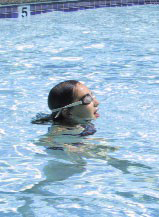
\includegraphics[scale=0.5]{src1.jpg}
	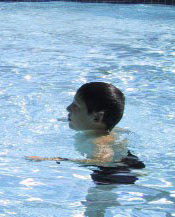
\includegraphics[scale=0.5]{src2.jpg}
	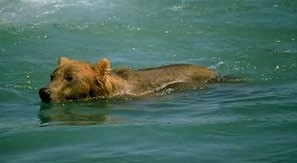
\includegraphics[scale=0.7]{src3.jpg}
}

	\noindent tgt: 	
	
	\centerline{	
	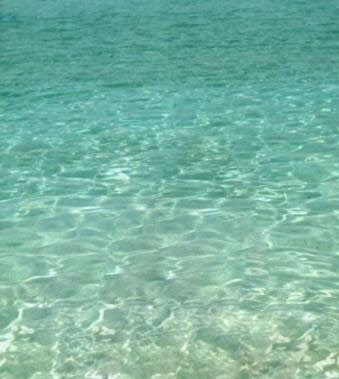
\includegraphics[scale=0.5]{tgt.jpg}
}
	
	\noindent mask: 
	
	\centerline{
		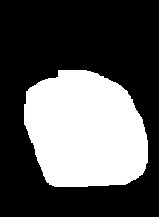
\includegraphics[scale=0.3]{mask1.jpg}
		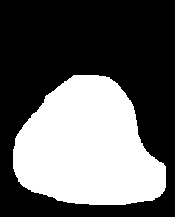
\includegraphics[scale=0.3]{mask2.jpg}
		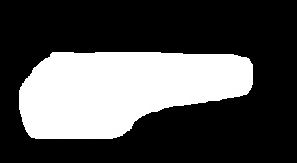
\includegraphics[scale=0.43]{mask3.jpg}
	}

	\noindent 输出:
	
	\centerline{	
	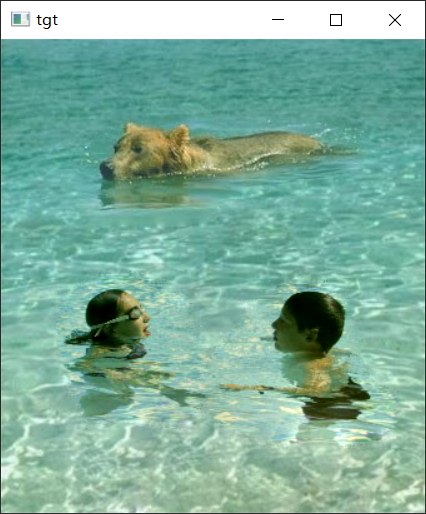
\includegraphics[scale=0.25]{Output1.png}
}
	
	\noindent 用时:4.13s
	\subsection{Mixing Gradient代码}
	梯度混合在原先的基础上对梯度进行了比较,因此在上述代码的基础上增加了几行代码,相同处不再给出,只给出67-68行的替代代码。
	\begin{lstlisting}
# 获取源图像和目标图像锚点和该方向上点的像素值
src_dir = p_src[old_row + direct[0], old_col + direct[1], :]
tgt_dir = p_tgt[row + direct[0], col + direct[1], :]
src_anc = p_src[old_row, old_col, :]
tgt_anc = p_tgt[row, col, :]

# 比较各方向梯度绝对值(三通道平方和开根),取较大的值
if np.linalg.norm(src_anc - src_dir) > np.linalg.norm(tgt_anc - tgt_dir):
	tmp_anc += (src_anc - src_dir)
else:
	tmp_anc += (tgt_anc - tgt_dir)
	\end{lstlisting}

	如果输入和上述相同的源图像、目标图像和掩膜,用时变为6.20s,相对于不采用梯度混合的方法增加了两秒,增加的时间主要用在梯度比较和行列式计算上。
	
	由于上述图像对目标图像的纹理显示不是十分明显,我们采用全新的输入图片。
	
	\noindent 输入:
	
	\noindent src: 
	
	\centerline{
		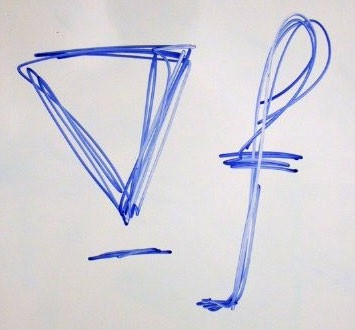
\includegraphics[scale=0.5]{2.jpg}
	}
	
	\noindent tgt: 	
	
	\centerline{	
		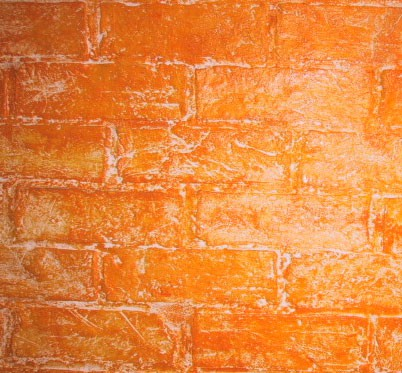
\includegraphics[scale=0.5]{1.jpg}
	}
	
	\noindent mask: 
	
	\centerline{
		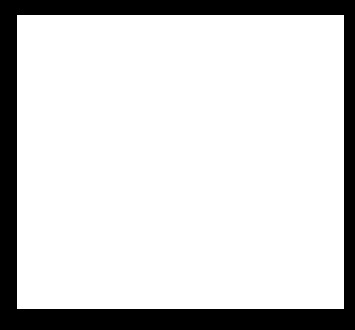
\includegraphics[scale=0.35]{mask.jpg}
	}
	
	\noindent 输出:
	
	\centerline{	
		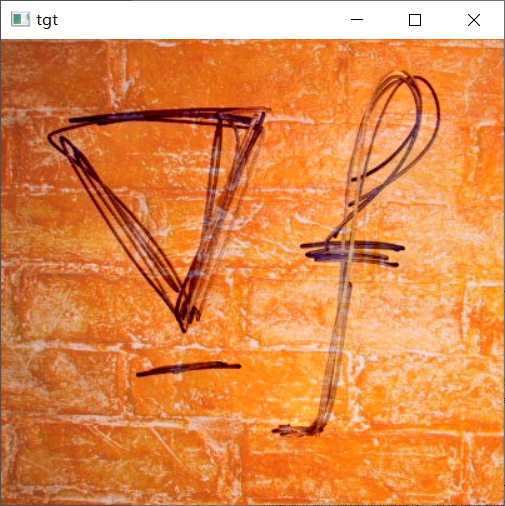
\includegraphics[scale=0.25]{Output2.png}
	}
	
	\noindent 用时:13.05s
	\section{参考内容}
	
	\noindent 文献:
	
	\hangafter = 1
	\hangindent 0.5in
	\noindent 
	Pérez, P., Gangnet, M., \& Blake, A. (2003). Poisson image editing. In \textsl{ACM SIGGRAPH 2003 Papers} (pp. 313-318).
	
	\noindent 网址:
	
	\noindent https://zhuanlan.zhihu.com/p/453095752
	
	\noindent https://zhuanlan.zhihu.com/p/356288730
	
	\noindent https://zhuanlan.zhihu.com/p/68349210
	
	\noindent https://blog.csdn.net/u010772377/article/details/119758184
	
\end{document}